\documentclass[
	9pt, % Set the default font size, options include: 8pt, 9pt, 10pt, 11pt, 12pt, 14pt, 17pt, 20pt
	t, % Uncomment to vertically align all slide content to the top of the slide, rather than the default centered
	%aspectratio=169, % Uncomment to set the aspect ratio to a 16:9 ratio which matches the aspect ratio of 1080p and 4K screens and projectors
]{beamer}

\graphicspath{{Images/}{./}} % Specifies where to look for included images (trailing slash required)

\usepackage{booktabs} % Allows the use of \toprule, \midrule and \bottomrule for better rules in tables
\usepackage{graphicx}
\usepackage{caption}
\usepackage{subcaption}
\usepackage{hyperref}
\usepackage[english,brazil]{babel}
\usepackage{fontawesome5}
\usepackage{listings}
\usepackage{minted}
\usepackage{xcolor}
% \usepackage{graphicx}
% \usepackage{animate}
\RequirePackage[backend=biber,
style=ieee,
citestyle=authoryear,
]{biblatex}

% Define a custom command for an icon link
\newcommand{\iconLink}[2]{\href{#1}{\faLink \hspace{0.2em} {#2}}}
\newcommand{\yellowbox}[1]{\colorbox{yellow!75}{#1}}
\definecolor{darkgreen}{rgb}{0,0.5,0}

% Definindo um estilo para o destaque
%----------------------------------------------------------------------------------------
%	SELECT LAYOUT THEME
%----------------------------------------------------------------------------------------
\usetheme{Madrid}

%----------------------------------------------------------------------------------------
%	SELECT COLOR THEME
%----------------------------------------------------------------------------------------

% Beamer comes with a number of color themes that can be applied to any layout theme to change its colors. Uncomment each of these in turn to see how they change the colors of your selected layout theme.

%\usecolortheme{albatross}
%\usecolortheme{beaver}
%\usecolortheme{beetle}
% \usecolortheme{crane}
%\usecolortheme{dolphin}
%\usecolortheme{dove}
%\usecolortheme{fly}
%\usecolortheme{lily}
%\usecolortheme{monarca}
%\usecolortheme{seagull}
%\usecolortheme{seahorse}
%\usecolortheme{spruce}
%\usecolortheme{whale}
%\usecolortheme{wolverine}

%----------------------------------------------------------------------------------------
%	SELECT FONT THEME & FONTS
%----------------------------------------------------------------------------------------
\usefonttheme{default} % Typeset using the default sans serif font

%------------------------------------------------

\usepackage{palatino} % Use the Palatino font for serif text
\usepackage[default]{lato} % Use the Lato font for sans serif text

%----------------------------------------------------------------------------------------
%	SELECT INNER THEME
%----------------------------------------------------------------------------------------
\useinnertheme{rectangles}

%----------------------------------------------------------------------------------------
%	SELECT OUTER THEME
%----------------------------------------------------------------------------------------

% Outer themes change the overall layout of slides, such as: header and footer lines, sidebars and slide titles. Uncomment each theme in turn to see what changes it makes to your presentation.

%\useoutertheme{default}
%\useoutertheme{infolines}
%\useoutertheme{miniframes}
%\useoutertheme{smoothbars}
%\useoutertheme{sidebar}
%\useoutertheme{split}
%\useoutertheme{shadow}
%\useoutertheme{tree}
%\useoutertheme{smoothtree}

%\setbeamertemplate{footline} % Uncomment this line to remove the footer line in all slides
%\setbeamertemplate{footline}[page number] % Uncomment this line to replace the footer line in all slides with a simple slide count

%\setbeamertemplate{navigation symbols}{} % Uncomment this line to remove the navigation symbols from the bottom of all slides

% \bibliography{references} % Specifies the bibliography file to include publications
% \bibliographystyle{apalike} % Specifies the bibliography style
\addbibresource{references.bib}

%----------------------------------------------------------------------------------------
%	PRESENTATION INFORMATION
%----------------------------------------------------------------------------------------

\title[DesWebII]{Desenvolvimento Web II} % The short title in the optional parameter appears at the bottom of every slide, the full title in the main parameter is only on the title page
\subtitle{Aula 11 - Web Components} % Presentation subtitle, remove this command if a subtitle isn't required
\author[Fabricio Bizotto]{Prof. Fabricio Bizotto} % Presenter name(s), the optional parameter can contain a shortened version to appear on the bottom of every slide, while the main parameter will appear on the title slide
\institute[IFC]{Instituto Federal Catarinense \\ \smallskip \textit{fabricio.bizotto@ifc.edu.br}} % Your institution, the optional parameter can be used for the institution shorthand and will appear on the bottom of every slide after author names, while the required parameter is used on the title slide and can include your email address or additional information on separate lines
\date[\today]{Ciência da Computação \\ \today} % Presentation date or conference/meeting name, the optional parameter can contain a shortened version to appear on the bottom of every slide, while the required parameter value is output to the title slide

%----------------------------------------------------------------------------------------
\begin{document}

%----------------------------------------------------------------------------------------
%	TITLE SLIDE
%----------------------------------------------------------------------------------------

\begin{frame}
	\titlepage % Output the title slide, automatically created using the text entered in the PRESENTATION INFORMATION block above
\end{frame}

%----------------------------------------------------------------------------------------
%	TABLE OF CONTENTS SLIDE
%----------------------------------------------------------------------------------------

\begin{frame}
	\frametitle{Roteiro} % Slide title, remove this command for no title
	
	\tableofcontents % Output the table of contents (all sections on one slide)
	%\tableofcontents[pausesections] % Output the table of contents (break sections up across separate slides)
\end{frame}

%----------------------------------------------------------------------------------------
%	PRESENTATION BODY SLIDES
%----------------------------------------------------------------------------------------

\section{Design System}

\begin{frame}
	\frametitle{Design System}
	\framesubtitle{Conceito}

	\begin{itemize}
		\item Design System é um conjunto de \yellowbox{padrões, práticas, diretrizes e componentes} que são usados para criar e manter produtos digitais.
		\item O objetivo é garantir a consistência e a qualidade do produto final.
		\item Um Design System inclui:
		\begin{itemize}
			\item \textbf{Componentes}: Botões, formulários, cards, etc.
			\item \textbf{Estilos}: Cores, tipografia, espaçamento, etc.
			\item \textbf{Padrões}: Diretrizes de uso, acessibilidade, etc.
		\end{itemize}
		\item Exemplos: Material Design, Bootstrap, Ant Design, Fast Design, Radix UI, GovBR-DS, etc.
		\item \textbf{Web Components são uma forma de criar e distribuir componentes em um Design System.}
	\end{itemize}

	\begin{figure}
		\centering
		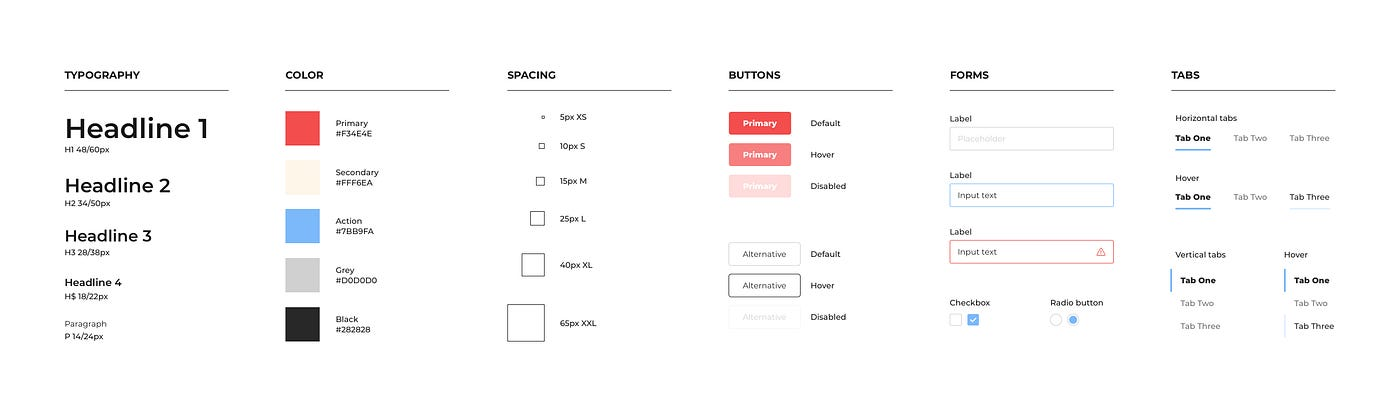
\includegraphics[width=0.9\textwidth]{design_system.jpg}
		\caption{Design System}
	\end{figure}

\end{frame}

\section{Web Components}

\begin{frame}
	\frametitle{Web Components}
	\framesubtitle{Conceito}
	\begin{itemize}
		\item Web Components são um conjunto de especificações elaboradas para permitir a criação de elementos web de forma customizada e independente.
		\item Web Components é uma especificação do W3C, que inclui:
		\begin{itemize}
			\item \textbf{Custom Elements}
			\item \textbf{Shadow DOM}
			\item \textbf{HTML Templates}
			\item \textbf{HTML Imports}
		\end{itemize}
		\item Frameworks como Angular, React e Vue.js ajudaram a popularizar a ideia de componentização no desenvolvimento web.
	\end{itemize}

	\begin{figure}
		\centering
		
\includegraphics[width=0.5\textwidth]{web_components.jpg}
		\caption{Web Components}
	\end{figure}

\end{frame}

\subsection{ciclo de vida}

\begin{frame}
	\frametitle{Web Components}
	\framesubtitle{Ciclo de Vida}
	\begin{itemize}
		\item Os Web Components têm um ciclo de vida que é gerenciado pelo navegador.
		\item O ciclo de vida é composto por callbacks que são chamados em diferentes momentos do ciclo de vida do componente.
		\item Os callbacks mais comuns são:
		\begin{itemize}
			\item \texttt{connectedCallback}: Chamado quando o componente é conectado ao DOM.
			\item \texttt{disconnectedCallback}: Chamado quando o componente é desconectado do DOM.
			\item \texttt{attributeChangedCallback}: Chamado quando um atributo do componente é alterado.
			\item \texttt{adoptedCallback}: Chamado quando o componente é movido para um novo documento.
		\end{itemize}
	\end{itemize}

\end{frame}

\begin{frame}
	\frametitle{Web Components}
	\framesubtitle{Custom Elements}
	\begin{itemize}
		\item Custom Elements é uma API que permite a criação de novos elementos HTML personalizados, encapsulando HTML, CSS e JavaScript.
		\item A classe pode ser estendida a partir de \texttt{HTMLElement} ou \texttt{HTMLButtonElement}, por exemplo.
	\end{itemize}

	\begin{figure}
		\centering
		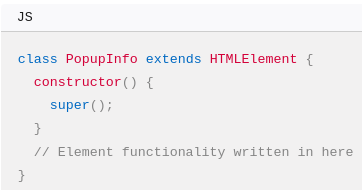
\includegraphics[width=0.5\textwidth]{custom_elements.png}
		\caption{Custom Elements}
	\end{figure}

\end{frame}

\subsection{DOM vs Shadow DOM}

\begin{frame}
	\frametitle{Web Components}
	\framesubtitle{DOM vs Shadow DOM}
	\begin{itemize}
		\item O DOM é uma árvore de elementos HTML/XML que representa a estrutura de uma página web. No contexto de Web Components, light DOM é o DOM padrão da página.
		\item O Shadow DOM é uma árvore de elementos HTML encapsulada que representa a estrutura de um componente web.
	\end{itemize}

	\begin{figure}
		\centering
		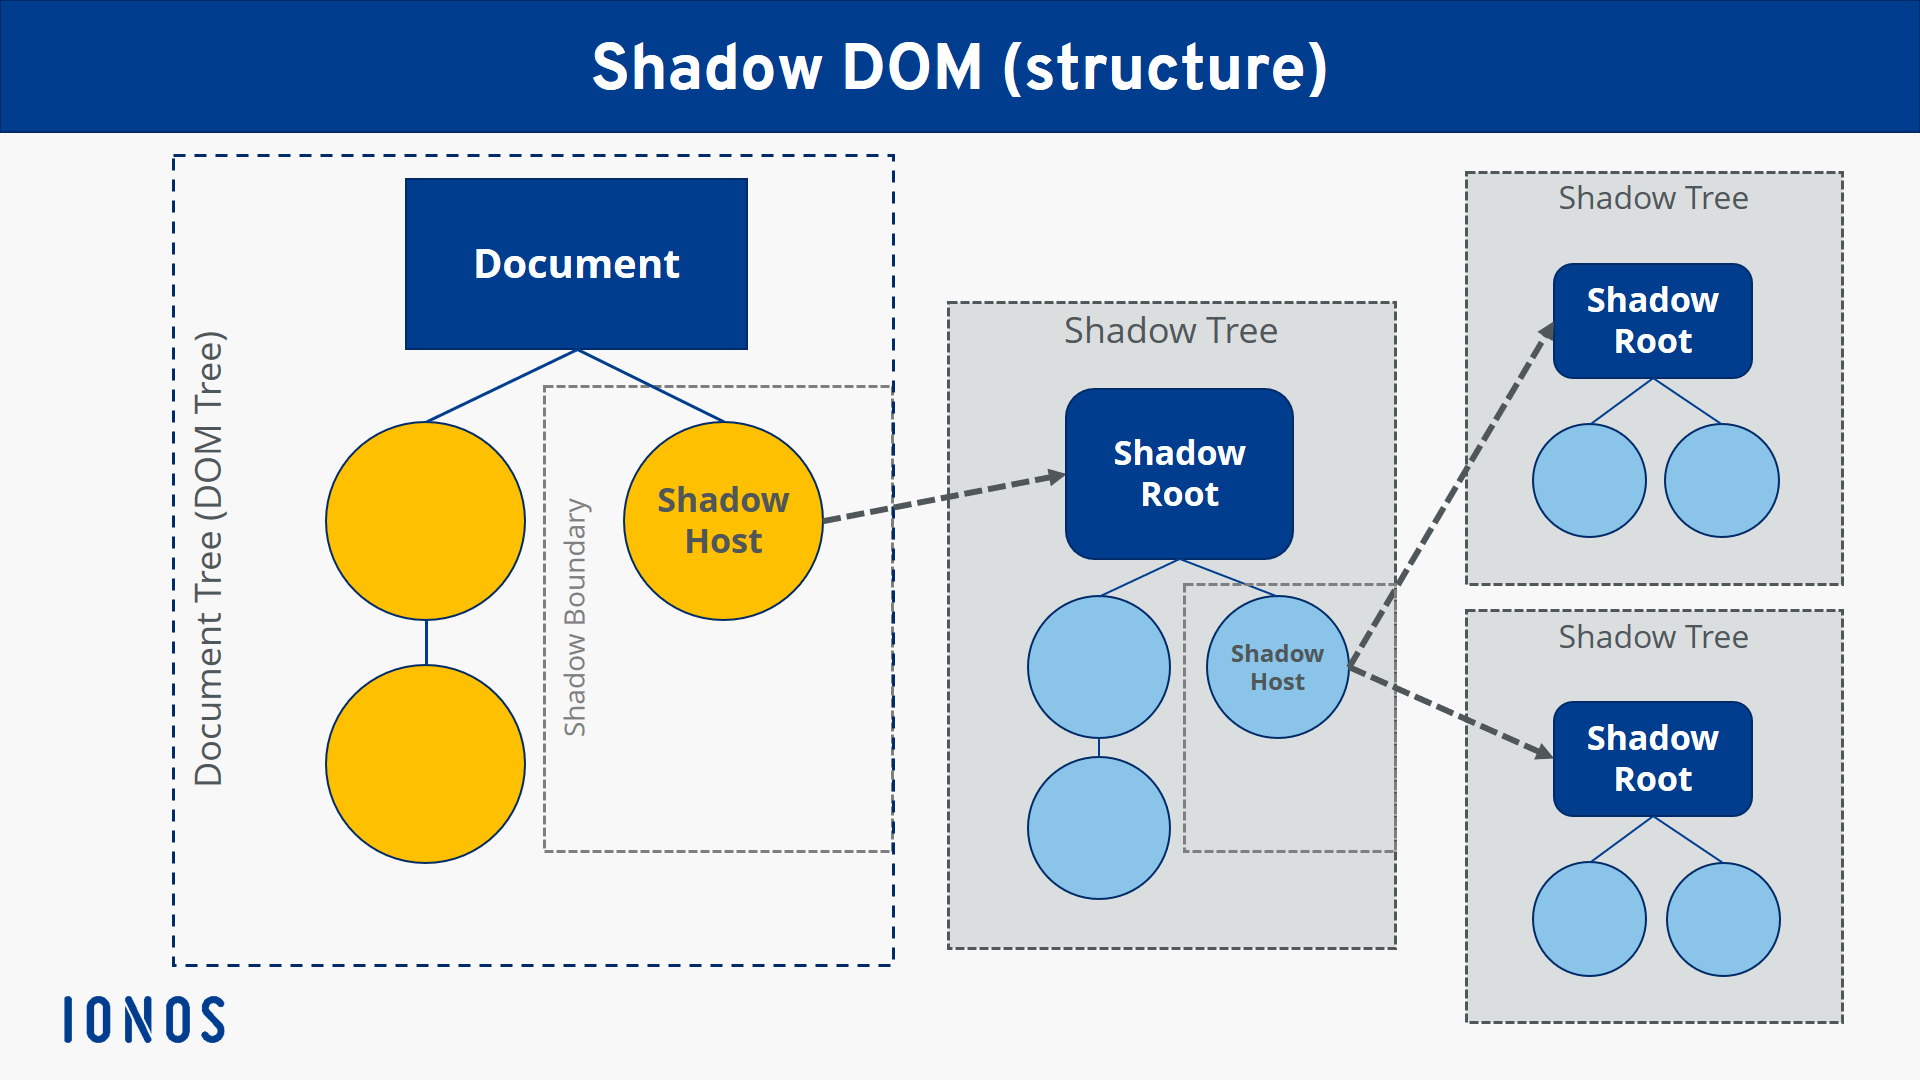
\includegraphics[width=0.7\textwidth]{dom_shadow_dom.png}
		\caption{DOM vs Shadow DOM}
	\end{figure}

\end{frame}

\begin{frame}
	\frametitle{Web Components}
	\framesubtitle{Shadow DOM}
	\begin{itemize}
		\item Shadow DOM é uma API que permite a criação de um DOM encapsulado para fornecer um encapsulamento de estilo e comportamento.
		\item Permite criar árvores de DOM independentes e isoladas que podem ser anexadas a um elemento HTML.
		\item Impede que estilos e scripts de fora do DOM encapsulado afetem o DOM encapsulado.
		\item Permite criar e reutilizar componentes.
		\item Exemplo: \texttt{<input type="range">} é um elemento nativo encapsulado.
	\end{itemize}

	\begin{figure}
		\centering
		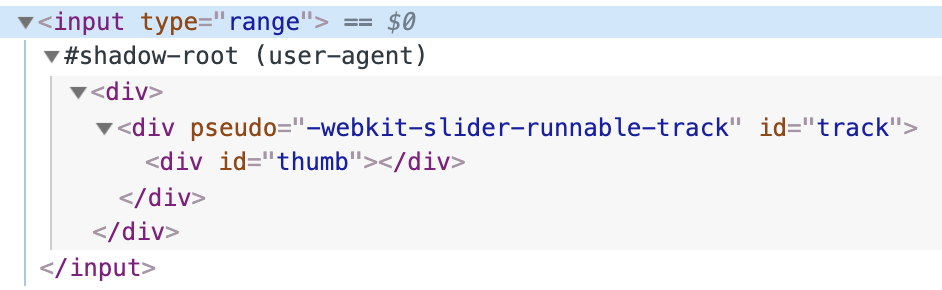
\includegraphics[width=0.8\textwidth]{shadow_dom_example.png}
		\caption{Shadow DOM - Exemplo}
	\end{figure}

\end{frame}

\subsection{HTML Templates e Slots}

\begin{frame}
	\frametitle{Web Components}
	\framesubtitle{HTML Templates}
	\begin{itemize}
		\item HTML Templates é uma tag que permite declarar fragmentos de código HTML que não são renderizados quando a página é carregada.
		\item O conteúdo do template pode ser clonado e renderizado posteriormente.
	\end{itemize}

	\begin{figure}
		\centering
		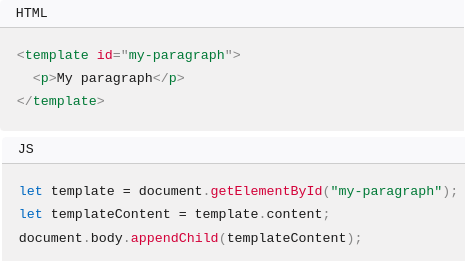
\includegraphics[width=0.8\textwidth]{html_templates.png}
		\caption{HTML Templates - Exemplo}
	\end{figure}

\end{frame}

\begin{frame}
	\frametitle{Web Components}
	\framesubtitle{HTML Templates - Slots}
	\begin{itemize}
		\item Slots são um mecanismo que permite inserir conteúdo dinâmico dentro de um componente encapsulado.
		\item Se um componente tem um slot, o conteúdo inserido no slot é renderizado no lugar do slot.
		\item O slot é usado para adicionar texto customizado.
	\end{itemize}

	\begin{figure}
		\centering
		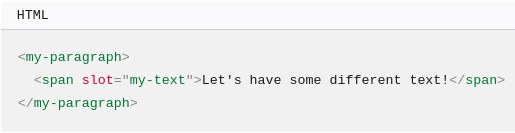
\includegraphics[width=0.8\textwidth]{html_slots.png}
		\caption{Slots - Exemplo}
	\end{figure}

\end{frame}

\subsection{HTML Imports - \textit{Descontinuado}}

\begin{frame}
	\frametitle{Web Components}
	\framesubtitle{HTML Imports}
	\begin{itemize}
		\item HTML Imports era uma especificação da W3C que permitia importar e incluir componentes web em outros documentos HTML.
		\item Foi descontinuado em favor de módulos ES6 que permitem importar e exportar módulos JavaScript.
	\end{itemize}

	\begin{block}{Exemplo}
		\texttt{// Importa o componente - \alert{descontinuado}}\\
		\texttt{<link rel=$"$import$"$ href=$"$component.html$"$>}\\

		\bigskip 
		\texttt{// Importa o módulo ES6}\\
		\texttt{import \{Component\} from $"$component.js$"$}
	\end{block}

\end{frame}

\section{Prós e Contras}

\begin{frame}
	\frametitle{Web Components}
	\framesubtitle{Prós e Contras}
	\begin{exampleblock}{Prós}
		\begin{itemize}
			\item \textbf{Reusabilidade}: Componentes podem ser reutilizados em diferentes projetos.
			\item \textbf{Encapsulamento}: O Shadow DOM permite encapsular estilos e comportamentos
			\item \textbf{Produtivididade}: Facilita a manutenção e evolução de aplicações web.
			\item \textbf{Padronização}: Padrão do W3C, suportado por todos os navegadores modernos.
		\end{itemize}
	\end{exampleblock}

	\begin{alertblock}{Contras}
		\begin{itemize}
			\item \textbf{Compatibilidade}: Não é suportado por navegadores mais antigos.
			\item \textbf{Complexidade}: Requer conhecimento avançado de HTML, CSS e JavaScript.
			\item \textbf{Performance}: Pode impactar a performance da aplicação.
			\item \textbf{Curva de Aprendizado}: Requer tempo para aprender e dominar.
			\item \textbf{Acessibilidade}: Pode impactar leitores de tela e outras tecnologias assistivas.
		\end{itemize}
	\end{alertblock}

\end{frame}

\section{Exemplo}

\begin{frame}
	\frametitle{Web Components}
	\framesubtitle{Exemplo}

	Para criar um Web Component, é necessário:
	\begin{itemize}
		\item Criar uma classe que estende \texttt{HTMLElement}
		\item Definir o template do componente
		\item Definir o Shadow DOM
		\item Registrar o componente
		\item Usar o componente
	\end{itemize}
	
	\begin{exampleblock}{Exemplo}
		\iconLink{https://gist.github.com/fabricioifc/36e978f4ff2add25ca0eed6e86219918}{Gist - Exemplo prático de Web Components}
	\end{exampleblock}	

\end{frame}

\section{Material Complementar}

\begin{frame}
	\frametitle{Web Components}
	\framesubtitle{Material Complementar}

	\begin{itemize}
		\item \iconLink{https://www.hipsters.tech/design-systems-hipsters-170/}{\textbf{Design System}}.\\Podcast - Hipsters \#170
		\item \iconLink{https://www.youtube.com/watch?v=PCWaFLy3VUo}{\textbf{Web Components}}.\\Vídeo - Web Components Crash Course
		\item \iconLink{https://youtu.be/7tsyjXxaloI?list=PL6BL1eKvLWOvfRhcDB0a5XJ2PD1_Rol6K}{\textbf{Componente de Ícone em SVG}}.\\Vídeo - Criando um Componente de Ícone
		\item \iconLink{https://www.webcomponents.org/introduction}{\textbf{Web Components - Introduction}}.\\Site - WebComponents.org
		\item \iconLink{https://ui.shadcn.com/}{\textbf{ShadCN - UI Components}}.\\Biblioteca de Componentes Web
		\item \iconLink{https://medium.com/@yourkube/10-best-web-component-libraries-b470541277e8}{\textbf{10 Best Web Component Libraries}}.\\Artigo - Medium
		\item \iconLink{https://webcomponent-ds.estaleiro.serpro.gov.br}{\textbf{Web Components - GovBR-DS}}.\\Design System do Governo Brasileiro
		\item \iconLink{https://ultimatecourses.com/blog/lifecycle-hooks-in-web-components}{\textbf{Lifecycle}}.\\Lifecycle Hooks in Web Components
	\end{itemize}

\end{frame}

\section{Experimento}

\begin{frame}
	\frametitle{Web Components}
	\framesubtitle{Experimento}

	Escolha dois dos seguintes exercícios para entregar até a próxima aula:

	\begin{enumerate}
		\item Crie um Web Component que represente um botão personalizado, com diferentes cores e tamanhos.
		\item Crie um Web Component para alterar o tema da página (claro/escuro).
		\item Crie um Web Component que represente um formulário de contato com campos de entrada para nome, e-mail, mensagem e um botão de envio.
		\item Crie um Web Component que represente um card com uma imagem, título e descrição.
		\item Crie um Web Component que represente um menu de navegação com links para diferentes páginas.
		\item Crie um Web Component que represente um carrossel de imagens.
		\item Outro componente de sua escolha.
	\end{enumerate}

	\begin{block}{Entrega}
		\begin{itemize}
			\item Crie um repositório no GitHub para entregar os exercícios.
			\item O componente precisa implementar o ciclo de vida.
			\item Crie um arquivo \texttt{README.md} com instruções sobre como usar os componentes.
		\end{itemize}
	\end{block}

\end{frame}

\end{document} 
